\subsection{Principle and solutions}

\begin{frame}
  \frametitle{Filesystems}
  \begin{itemize}
  \item Filesystems are used to organize data in directories and files
    on storage devices or on the network. The directories and files
    are organized as a hierarchy
  \item In UNIX systems, applications and users see a {\bf single
      global hierarchy} of files and directories, which can be
    composed of several filesystems.
  \item Filesystems are {\bf mounted} in a specific location in this
    hierarchy of directories
    \begin{itemize}
    \item When a filesystem is mounted in a directory (called {\em
        mount point}), the contents of this directory reflect the
        contents of this filesystem.
    \item When the filesystem is unmounted, the {\em mount point} is
      empty again.
    \end{itemize}
  \item This allows applications to access files and directories easily,
    regardless of their exact storage location
  \end{itemize}
\end{frame}

\begin{frame}
  \frametitle{Filesystems (2)}
  \begin{itemize}
  \item Create a mount point, which is just a directory\\
    \code{$ sudo mkdir /mnt/usbkey}
  \item It is empty\\
    \code{$ ls /mnt/usbkey}\\
    \code{$}
  \item Mount a storage device in this mount point\\
    \code{$ sudo mount -t vfat /dev/sda1 /mnt/usbkey}\\
    \code{$}
  \item You can access the contents of the USB key\\
    \code{$ ls /mnt/usbkey}\\
    \code{docs prog.c picture.png movie.avi}\\
    \code{$}
  \end{itemize}
\end{frame}

\begin{frame}
  \frametitle{mount / umount}
  \begin{itemize}
  \item \code{mount} allows to mount filesystems
    \begin{itemize}
    \item \code{mount -t type device mountpoint}
    \item \code{type} is the type of filesystem (optional for
	non-virtual filesystems)
    \item \code{device} is the storage device, or network location to
      mount
    \item \code{mountpoint} is the directory where files of the
      storage device or network location will be accessible
    \item \code{mount} with no arguments shows the currently mounted
      filesystems
    \end{itemize}
  \item \code{umount} allows to unmount filesystems
    \begin{itemize}
    \item This is needed before rebooting, or before unplugging a USB
      key, because the Linux kernel caches writes in memory to
      increase performance. \code{umount} makes sure that these writes are
      committed to the storage.
    \end{itemize}
  \end{itemize}
\end{frame}

\begin{frame}[fragile]
  \frametitle{Root filesystem}
  \begin{itemize}
  \item A particular filesystem is mounted at the root of the hierarchy,
    identified by \code{/}
  \item This filesystem is called the {\bf root filesystem}
  \item As \code{mount} and \code{umount} are programs, they are files
    inside a filesystem.
    \begin{itemize}
    \item They are not accessible before mounting at least one filesystem.
    \end{itemize}
  \item As the root filesystem is the first mounted filesystem, it
    cannot be mounted with the normal \code{mount} command
  \item It is mounted directly by the kernel, according to the
    \code{root=} kernel option
  \item When no root filesystem is available, the kernel panics:\\
    \small
\begin{verbatim}
Please append a correct "root=" boot option
Kernel panic - not syncing: VFS: Unable to mount root fs on unknown block(0,0)
\end{verbatim}
  \end{itemize}
\end{frame}

\begin{frame}
  \frametitle{Location of the root filesystem}
  \begin{itemize}
  \item It can be mounted from different locations
    \begin{itemize}
    \item From the partition of a hard disk
    \item From the partition of a USB key
    \item From the partition of an SD card
    \item From the partition of a NAND flash chip or similar type of
      storage device
    \item From the network, using the NFS protocol
    \item From memory, using a pre-loaded filesystem (by the
      bootloader)
    \item etc.
    \end{itemize}
  \item It is up to the system designer to choose the configuration
    for the system, and configure the kernel behavior with
    \code{root=}
  \end{itemize}
\end{frame}

\begin{frame}
  \frametitle{Mounting rootfs from storage devices}
  \begin{itemize}
  \item Partitions of a hard disk or USB key
    \begin{itemize}
    \item \code{root=/dev/sdXY}, where \code{X} is a letter indicating
      the device, and \code{Y} a number indicating the partition
    \item \code{/dev/sdb2} is the second partition of the second disk
      drive (either USB key or ATA hard drive)
    \end{itemize}
  \item Partitions of an SD card
    \begin{itemize}
    \item \code{root=/dev/mmcblkXpY}, where \code{X} is a number
      indicating the device and \code{Y} a number indicating the
      partition
    \item \code{/dev/mmcblk0p2} is the second partition of the first
      device
    \end{itemize}
  \item Partitions of flash storage
    \begin{itemize}
    \item \code{root=/dev/mtdblockX}, where \code{X} is the partition number
    \item \code{/dev/mtdblock3} is the fourth enumerated flash partition in the system
	  (there could be multiple flash chips)
    \end{itemize}
  \end{itemize}
\end{frame}

\begin{frame}
  \frametitle{Mounting rootfs over the network (1)}

  Once networking works, your root filesystem could be a directory on
  your GNU/Linux development host, exported by NFS (Network File
  System). This is very convenient for system development:

  \begin{itemize}
  \item Makes it very easy to update files on the root filesystem,
    without rebooting.
  \item Can have a big root filesystem even if you don't have support
    for internal or external storage yet.
  \item The root filesystem can be huge. You can even build native
    compiler tools and build all the tools you need on the target
    itself (better to cross-compile though).
  \end{itemize}

  \begin{center}
    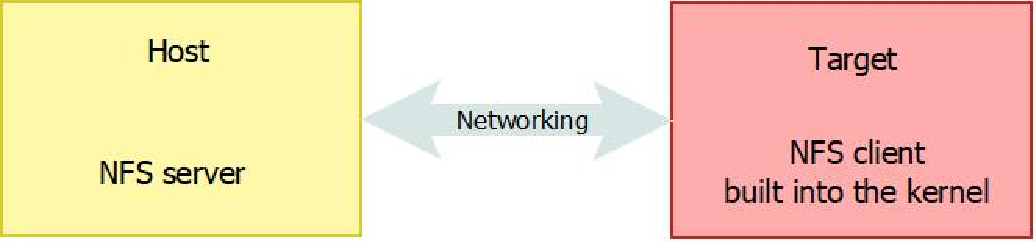
\includegraphics[width=0.7\textwidth]{slides/sysdev-root-filesystem-principles/nfs-principle.pdf}
  \end{center}
\end{frame}

\begin{frame}
  \frametitle{Mounting rootfs over the network (2)}

  On the development workstation side, a NFS server is needed

  \begin{itemize}
  \item Install an NFS server (example: Debian, Ubuntu)\\
    \code{sudo apt install nfs-kernel-server}
  \item Add the exported directory to your \code{/etc/exports} file:\\
    \code{/home/tux/rootfs 192.168.1.111(rw,no_root_squash,no_subtree_check)}
    \begin{itemize}
    \item \code{192.168.1.111} is the client IP address
    \item \code{rw,no_root_squash,no_subtree_check} are the NFS server
      options for this directory export.
    \end{itemize}
  \item Ask your NFS server to reload this file:\\
    \code{sudo exportfs -r}
  \end{itemize}
\end{frame}

\begin{frame}
  \frametitle{Mounting rootfs over the network (3)}
  \begin{itemize}
  \item On the target system
  \item The kernel must be compiled with
    \begin{itemize}
    \item \kconfigval{CONFIG_NFS_FS}{y} (NFS {\bf client} support)
    \item \kconfigval{CONFIG_ROOT_NFS}{y} (support for NFS as rootfs)
    \item \kconfigval{CONFIG_IP_PNP}{y} (configure IP at boot time)
    \end{itemize}
  \item The kernel must be booted with the following parameters:
    \begin{itemize}
    \item \code{root=/dev/nfs} (we want rootfs over NFS)
    \item \code{ip=192.168.1.111} (target IP address)
    \item \code{nfsroot=192.168.1.110:/home/tux/rootfs/} (NFS server details)
    \item You may need to add "\code{,nfsvers=3,tcp}" to the
      \code{nfsroot} setting, as an NFS version 2 client and UDP may
      be rejected by the NFS server in recent GNU/Linux distributions.
    \end{itemize}
  \end{itemize}
\end{frame}

\begin{frame}
  \frametitle{Mounting rootfs over the network (4)}
  \begin{center}
    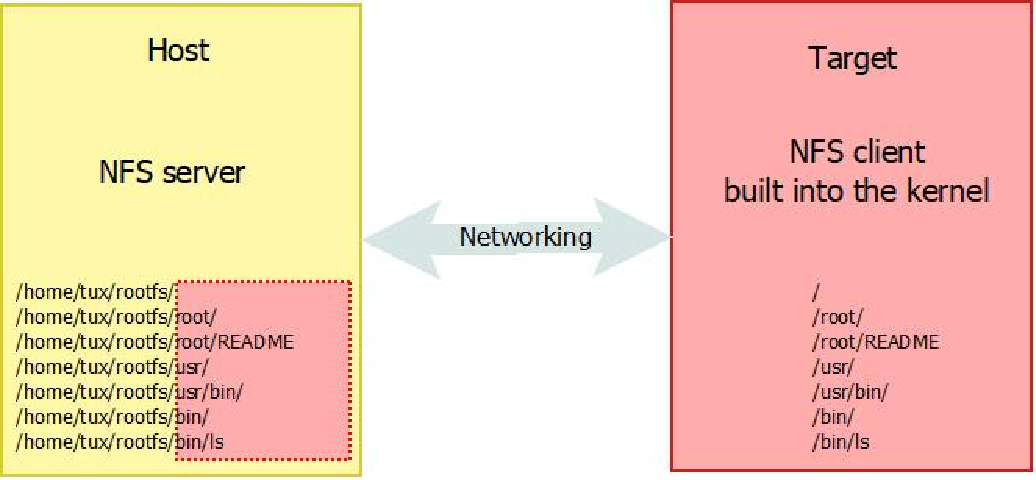
\includegraphics[width=0.9\textwidth]{slides/sysdev-root-filesystem-principles/nfs-principle-with-details.pdf}
  \end{center}
\end{frame}
